\documentclass[11pt]{article}
\usepackage[margin=1in]{geometry}
\usepackage{booktabs}
\usepackage{array}
\usepackage{longtable}
\usepackage{amsmath}
\usepackage{graphicx}
\usepackage{caption}
\usepackage{float}
\usepackage[table]{xcolor}
\usepackage{tikz}
\usetikzlibrary{arrows.meta,positioning,backgrounds,fit}
\usepackage[hidelinks]{hyperref}
\definecolor{vgreen}{HTML}{1B7837}
\definecolor{vorange}{HTML}{C97A0A}
\definecolor{vred}{HTML}{C0392B}
\definecolor{vgray}{HTML}{555555}
\definecolor{fd1c}{HTML}{1f77b4}
\definecolor{fd3c}{HTML}{C0392B}
\newcommand{\ttt}[1]{\texttt{#1}}
\newcommand{\verd}[2]{\textcolor{#1}{\textbf{#2}}}
\setlength{\parindent}{0pt}
\setlength{\parskip}{0.55em}


\begin{document}

\title{\textbf{Which cells are FD2 and FD3? A connectomic assignment of \ttt{LPT21}, \ttt{Nod3} and \ttt{LPT42\_Nod4}}}

\author{Stage 10 FD2/FD3 Disambiguation}

\date{\today}

\maketitle

\tableofcontents

\textbf{Summary.}\quad Three cell types in the fly connectome are regressive, cholinergic, noduli-family figure cells: \ttt{LPT42\_Nod4}, \ttt{Nod3}, and \ttt{LPT21}. Egelhaaf described two regressive figure-detection cells, FD2 and FD3, which share a preferred direction but differ in receptive field and projection side. This report measures the distinguishing properties for all three candidates and assigns each. \ttt{LPT42\_Nod4} is FD3: its receptive field sits laterally with a frontal gap and 90.33\% of its output crosses the midline (heterolateral). \ttt{LPT21} is FD2: its receptive field is frontal, co-located with the FD1 cell, and its output is almost entirely on its own side (1.48\% contralateral), the homolateral projection to the ipsilateral posterior optic foci that Egelhaaf reported for FD2. \ttt{Nod3} is neither cleanly: it is regressive but its output is mixed (44.66\% contralateral) and its field is only slightly lateral, so it sits between FD2 and FD3 and is left as an intermediate rather than forced into one identity. The primary numbers come from the offline v783 track; the laterality measurements are confirmed on the live and v630 tracks. Each cell type is a single bilateral pair, so the result rests on left-right agreement and on the thousands of synapses per cell, not on a population average.

\section{Introduction}

\textbf{Figure-ground discrimination and the FD cells.}\quad
A textured object is invisible against a matched background until it moves at a different velocity or
phase; relative motion then makes it salient. Reichardt and Poggio showed behaviourally that flies
detect and track such figures~\cite{rp1979}. Egelhaaf, in a three-part study, described the neurons
that could implement this~\cite{egelhaaf1985a,egelhaaf1985b,egelhaaf1985c}. Part~II defined a class of
lobula-plate tangential cells, the \emph{figure-detection} (FD) cells, each responding more strongly
to a small moving figure than to wide-field motion. Two of them are excited by \emph{regressive}
(back-to-front) motion. \textbf{FD2} has a frontal excitatory field (peak azimuth $0$--$10^\circ$,
reaching the frontal margin of the eye) and is a homolateral cell whose axon projects to the
\emph{ipsilateral} posterior optic foci; Egelhaaf notes it is not a ``noduli-group'' cell and that its
large-field organisation could not be resolved~\cite[p.~201]{egelhaaf1985b}. \textbf{FD3} has a
fronto-lateral field (peak $40$--$50^\circ$) that alone among the FD cells spares the most-frontal
$10$--$20^\circ$ (a frontal gap), and it is a heterolateral ``noduli-group'' cell whose axon crosses
the midline posterior to the noduli to the \emph{contralateral} posterior optic
foci~\cite[p.~202--204]{egelhaaf1985b}. The two regressive cells therefore share a preferred direction
and differ on two axes: the receptive field (frontal versus fronto-lateral with a gap) and the
projection side (homolateral/ipsilateral versus heterolateral/contralateral).

\textbf{The three candidates.}\quad
FD1 has already been mapped to the cholinergic cell type \ttt{Nod1}, which reads front-to-back
motion~\cite{maisak2013,fd1989}. Among the remaining noduli-family cells, three are regressive and
cholinergic: \ttt{LPT42\_Nod4}, \ttt{Nod3}, and \ttt{LPT21}. Because they share direction and
transmitter, those properties cannot assign them; the assignment rests on the receptive field and the
projection side. This report measures both for all three, together with the small-field selectivity,
the morphology, and the whole-family feature match, and reads off each cell's Egelhaaf identity.

\textbf{How the assignment is made.}\quad
Each distinguishing property is measured directly in the connectome: the projection side from where a
cell's output synapses land, the receptive field from the retinotopic positions of its motion inputs
relative to the frontal FD1 cell, and the axon path from the cell's reconstructed shape. We measure
these for all three candidates, on both cells of each bilateral pair, on the offline (primary), live,
and v630 tracks. The receptive-field comparison is made relative to the FD1=\ttt{Nod1} anchor in the
same coordinate frame, so it needs no conversion into visual angle. Figure~\ref{fig:concept} fixes the
FD2-versus-FD3 distinction; the sections that follow take each property in turn.

\begin{figure}[H]\centering
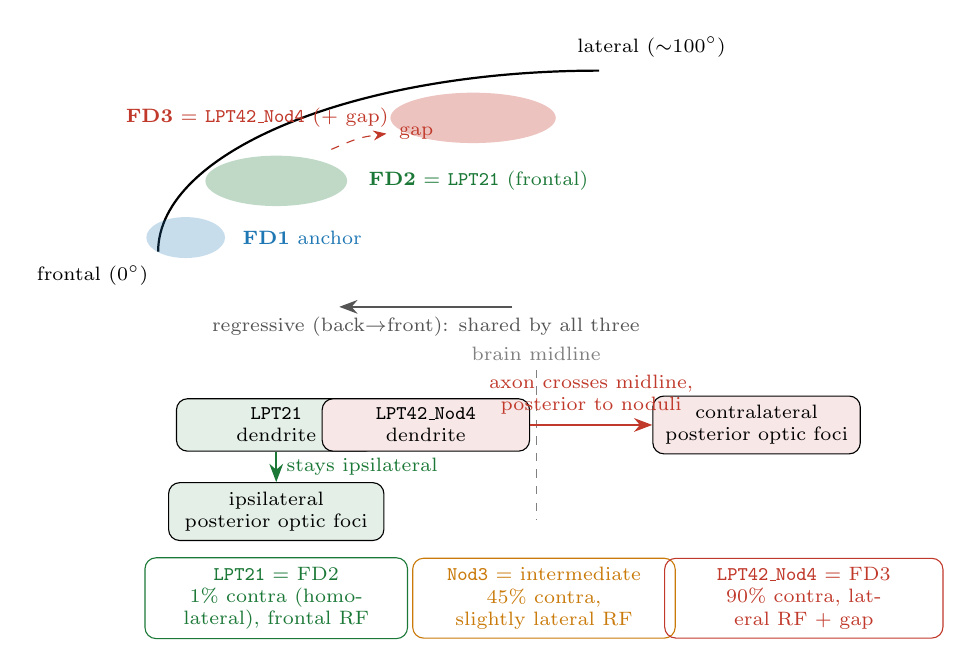
\begin{tikzpicture}[font=\small,>=Stealth]
  % ---- top: receptive fields on a shared visual-field arc ----
  \draw[thick] (0,0) arc (180:90:5.6 and 2.3);
  \node[anchor=north east,font=\scriptsize] at (0,-0.05) {frontal ($0^\circ$)};
  \node[anchor=south west,font=\scriptsize] at (5.2,2.35) {lateral ($\sim$100$^\circ$)};
  \fill[fd1c,opacity=0.25] (0.35,0.18) ellipse (0.5 and 0.26);
  \node[fd1c,font=\scriptsize,anchor=west] at (0.95,0.18) {\textbf{FD1} anchor};
  % FD2 (LPT21): frontal field, fills the frontal band
  \fill[vgreen,opacity=0.28] (1.5,0.9) ellipse (0.9 and 0.32);
  \node[vgreen,font=\scriptsize,anchor=west] at (2.55,0.9) {\textbf{FD2} $=$ \ttt{LPT21} (frontal)};
  % FD3 (LPT42_Nod4): fronto-lateral field with a gap
  \fill[fd3c,opacity=0.30] (4.0,1.7) ellipse (1.05 and 0.32);
  \node[fd3c,font=\scriptsize,anchor=east] at (3.05,1.7) {\textbf{FD3} $=$ \ttt{LPT42\_Nod4} ($+$ gap)};
  \draw[fd3c,dashed,->] (2.2,1.3) .. controls (2.55,1.45) .. (2.9,1.5)
        node[right,fd3c,font=\scriptsize,xshift=1pt]{gap};
  \draw[->,thick,vgray] (4.5,-0.7) -- (2.3,-0.7)
        node[midway,below,font=\scriptsize]{regressive (back$\to$front): shared by all three};
  % ---- bottom: projection, split by a dashed midline ----
  \draw[dashed,gray] (4.8,-1.5) -- (4.8,-3.4);
  \node[gray,font=\scriptsize,anchor=south] at (4.8,-1.5) {brain midline};
  \node[draw,rounded corners,fill=vgreen!12,font=\scriptsize,align=center,text width=2.3cm]
        (fd2d) at (1.5,-2.2) {\ttt{LPT21}\\dendrite};
  \node[draw,rounded corners,fill=vgreen!12,font=\scriptsize,align=center,text width=2.5cm]
        (fd2a) at (1.5,-3.3) {ipsilateral\\posterior optic foci};
  \draw[->,thick,vgreen] (fd2d) -- node[right,font=\scriptsize]{stays ipsilateral} (fd2a);
  \node[draw,rounded corners,fill=fd3c!12,font=\scriptsize,align=center,text width=2.4cm]
        (fd3d) at (3.4,-2.2) {\ttt{LPT42\_Nod4}\\dendrite};
  \node[draw,rounded corners,fill=fd3c!12,font=\scriptsize,align=center,text width=2.4cm]
        (fd3a) at (7.6,-2.2) {contralateral\\posterior optic foci};
  \draw[->,thick,fd3c] (fd3d) -- node[above,midway,font=\scriptsize,align=center]
        {axon crosses midline,\\posterior to noduli} (fd3a);
  % ---- candidate tags ----
  \node[draw,rounded corners,vgreen,font=\scriptsize,align=center,text width=3.1cm]
        at (1.5,-4.4) {\ttt{LPT21} $=$ FD2\\1\% contra (homolateral), frontal RF};
  \node[draw,rounded corners,vorange,font=\scriptsize,align=center,text width=3.1cm]
        at (4.9,-4.4) {\ttt{Nod3} $=$ intermediate\\45\% contra, slightly lateral RF};
  \node[draw,rounded corners,fd3c,font=\scriptsize,align=center,text width=3.3cm]
        at (8.2,-4.4) {\ttt{LPT42\_Nod4} $=$ FD3\\90\% contra, lateral RF $+$ gap};
\end{tikzpicture}
\caption{\textbf{Three regressive figure-detection candidates, and which Egelhaaf cell each is.}
Egelhaaf's FD2 and FD3 are both excited by regressive (back-to-front) motion, so direction alone
cannot tell them apart. They differ in receptive field and projection side: FD2 has a frontal field
and a homolateral axon to the ipsilateral posterior optic foci; FD3 has a fronto-lateral field with a
frontal gap and a heterolateral axon that crosses the midline posterior to the noduli. The connectome
places \ttt{LPT21} at FD2 (frontal field, essentially all output ipsilateral), \ttt{LPT42\_Nod4} at
FD3 (fronto-lateral field with a gap, output contralateral), and \ttt{Nod3} between them (a mixed
projection and a slightly lateral field), so \ttt{Nod3} is not a clean match to either.}%
\label{fig:concept}
\end{figure}


\section{The assignment rule}

Two Egelhaaf properties separate the regressive figure cells, and each maps onto a connectome
measurement. \textbf{FD3} requires a fronto-lateral receptive field with a frontal gap (its field sits
lateral of the frontal FD1 cell and vacates the frontal band) \emph{and} a heterolateral axon (the
large majority of its output crosses the midline). \textbf{FD2} requires a frontal receptive field
(co-located with the frontal FD1 cell, filling the frontal band, no gap) \emph{and} a homolateral axon
(its output stays on its own side, the ipsilateral projection). A cell that is regressive but matches
neither pattern cleanly, sitting between the two on both axes, is left as an intermediate rather than
forced into an identity.

The rule can conclude differently for each candidate and is not tuned to a desired answer. \ttt{LPT42\_Nod4}
is assigned FD3 when it has the lateral field with a gap and the heterolateral axon; \ttt{LPT21} is
assigned FD2 when it has the frontal field and the homolateral axon; and \ttt{Nod3} is assigned an
identity only if it matches one pattern cleanly. The single most important point of method is that
output laterality is measured on a continuum rather than a single threshold: a homolateral cell (FD2)
keeps its output near zero percent contralateral, a heterolateral cell (FD3) sends most output across,
and a cell in between is neither. This is what distinguishes \ttt{LPT21} (homolateral) from \ttt{Nod3}
(mixed), a distinction a single heterolateral cut-off would miss.

\section{Evidence, property by property}

We take the properties in turn: first the ones all three candidates share, which cannot assign them, then the two axes that separate FD2 from FD3.

\paragraph{All three cells prefer regressive motion, so direction cannot assign them.} A cell's preferred direction is read from which lobula-plate layer its motion inputs come from. \ttt{LPT21} draws 99.17\% of its motion input from the back-to-front layer, \ttt{Nod3} 97.73\%, and \ttt{LPT42\_Nod4} 98.58\% (Fig.~\ref{fig:layers}). All three are regressive, as both FD2 and FD3 are, so this property is shared and assigns none of them.

\begin{figure}[H]\centering
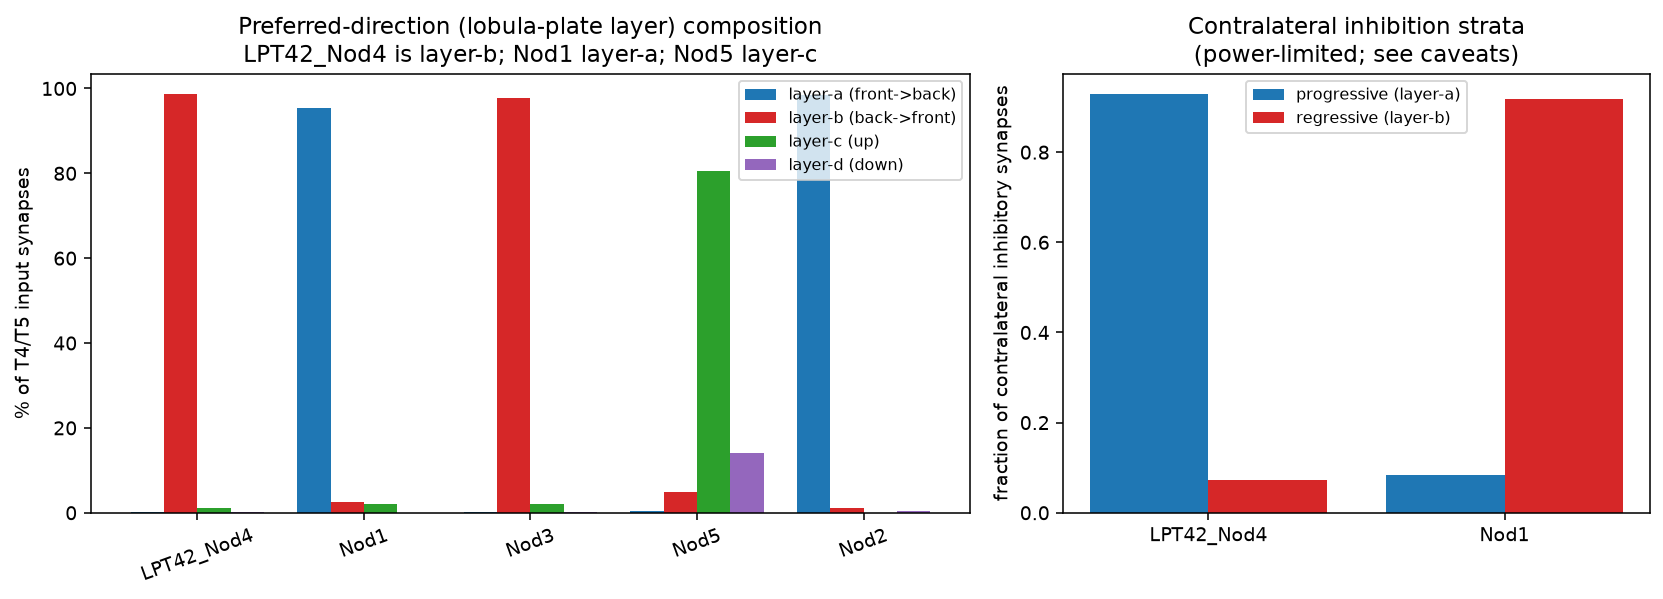
\includegraphics[width=\textwidth]{figures/fd3_layer_composition.png}
\caption{\textbf{Preferred direction is shared.} The share of each cell's motion input from the four directional layers. \ttt{LPT42\_Nod4}, \ttt{Nod3} and \ttt{Nod1} are shown here (the layer profile of \ttt{LPT21} is likewise almost entirely back-to-front). Because FD2 and FD3 are both regressive, this panel does not separate the candidates.}\label{fig:layers}
\end{figure}


\paragraph{All three are cholinergic, so transmitter cannot assign them.} Each releases acetylcholine (\ttt{LPT21} confidence 0.8132, \ttt{Nod3} 0.8784, \ttt{LPT42\_Nod4} 0.8943), and each is classified as a visual output neuron. Transmitter and cell class are therefore also shared.

\paragraph{Projection side: \ttt{LPT21} homolateral, \ttt{LPT42\_Nod4} heterolateral, \ttt{Nod3} mixed.} Egelhaaf's FD2 is a homolateral cell whose axon projects to the ipsilateral posterior optic foci, whereas FD3 is heterolateral, its axon crossing to the contralateral side. In the connectome \ttt{LPT21} sends only 1.48\% of its output across the midline, the clean homolateral projection of FD2; \ttt{LPT42\_Nod4} sends 90.33\%, the heterolateral projection of FD3; and \ttt{Nod3} sends 44.66\%, neither on its own side nor predominantly across, a mixed projection that matches FD2's homolateral anatomy no better than FD3's heterolateral one (Fig.~\ref{fig:contra}).

\paragraph{The projection ordering holds on every data track.} The fraction of output that is contralateral is sensitive to the data source, so it is reported on more than one track. On the live track \ttt{LPT21} is 1.58\%, \ttt{Nod3} 39.19\%, and \ttt{LPT42\_Nod4} 80.47\%. The exact numbers move between tracks, but the ordering, \ttt{LPT21} lowest, \ttt{LPT42\_Nod4} highest, \ttt{Nod3} in between, is preserved.

\begin{figure}[H]\centering
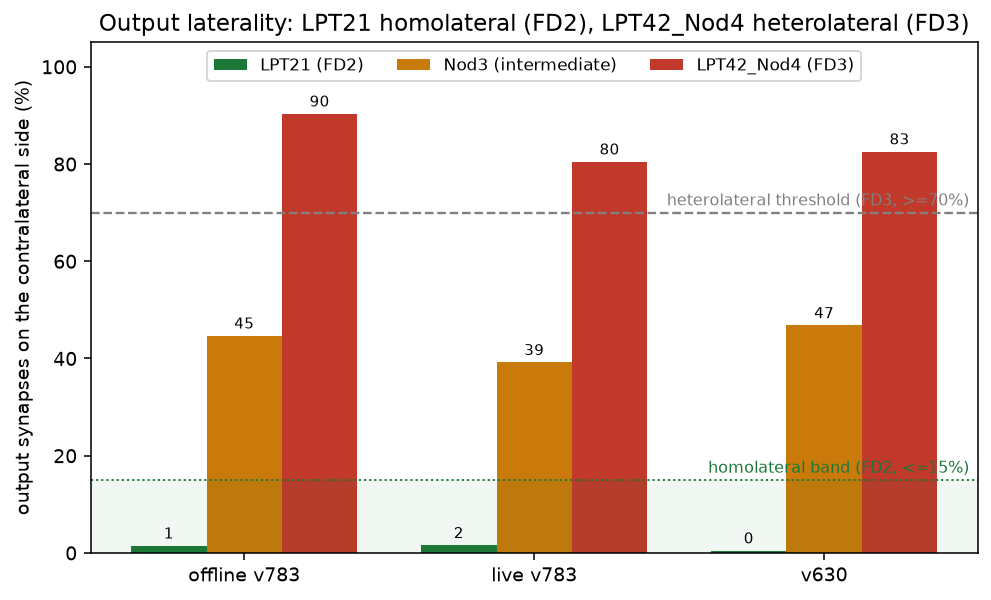
\includegraphics[width=\textwidth]{figures/fd3_disambig_contra.png}
\caption{\textbf{Output laterality.} The fraction of each candidate's output synapses on the contralateral side, on the offline, live and v630 tracks. \ttt{LPT21} lies in the homolateral band (near zero, the FD2 projection); \ttt{LPT42\_Nod4} clears the heterolateral threshold (the FD3 projection); \ttt{Nod3} sits between them.}\label{fig:contra}
\end{figure}


\paragraph{Receptive field: \ttt{LPT21} frontal, \ttt{LPT42\_Nod4} lateral with a gap, \ttt{Nod3} slightly lateral.} Measured against the frontal FD1 cell in the same coordinate frame, the field of \ttt{LPT21} is co-located with FD1 and fills the frontal band, the frontal field Egelhaaf reported for FD2. The field of \ttt{LPT42\_Nod4} sits far to the side and vacates the frontal band, the fronto-lateral field with a frontal gap that defines FD3. The field of \ttt{Nod3} is displaced only a few columns from the front and keeps most of its frontal occupancy, so it is neither clearly frontal nor clearly lateral (Fig.~\ref{fig:rf}).

\begin{figure}[H]\centering
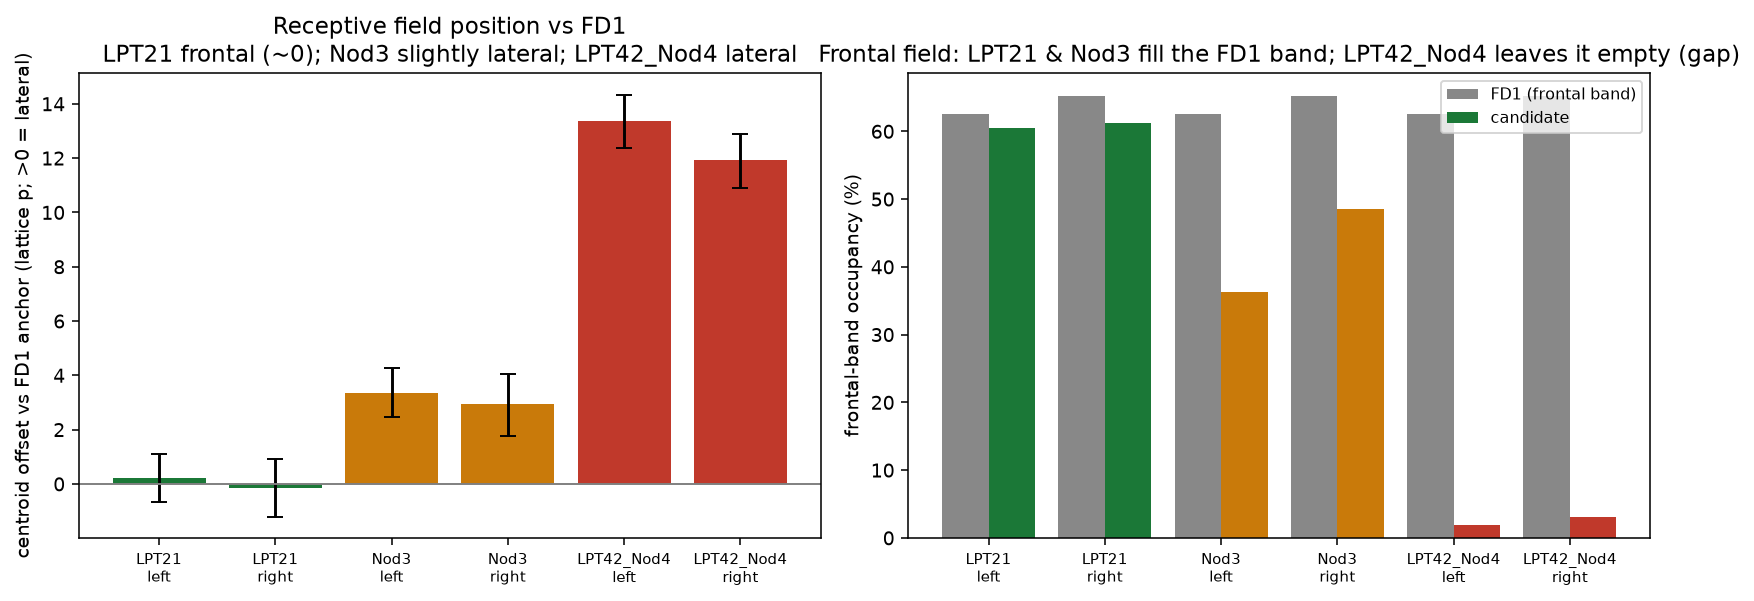
\includegraphics[width=\textwidth]{figures/fd3_disambig_rf.png}
\caption{\textbf{Receptive field position and the frontal gap.} (left) The centroid of each candidate's input field relative to the frontal FD1 anchor, per side, with $95\%$ confidence intervals: \ttt{LPT21} near zero (frontal), \ttt{Nod3} a few columns lateral, \ttt{LPT42\_Nod4} far lateral. (right) Frontal-band occupancy: \ttt{LPT21} and \ttt{Nod3} fill the FD1 band, \ttt{LPT42\_Nod4} leaves it nearly empty (the gap).}\label{fig:rf}
\end{figure}


\begin{figure}[H]\centering
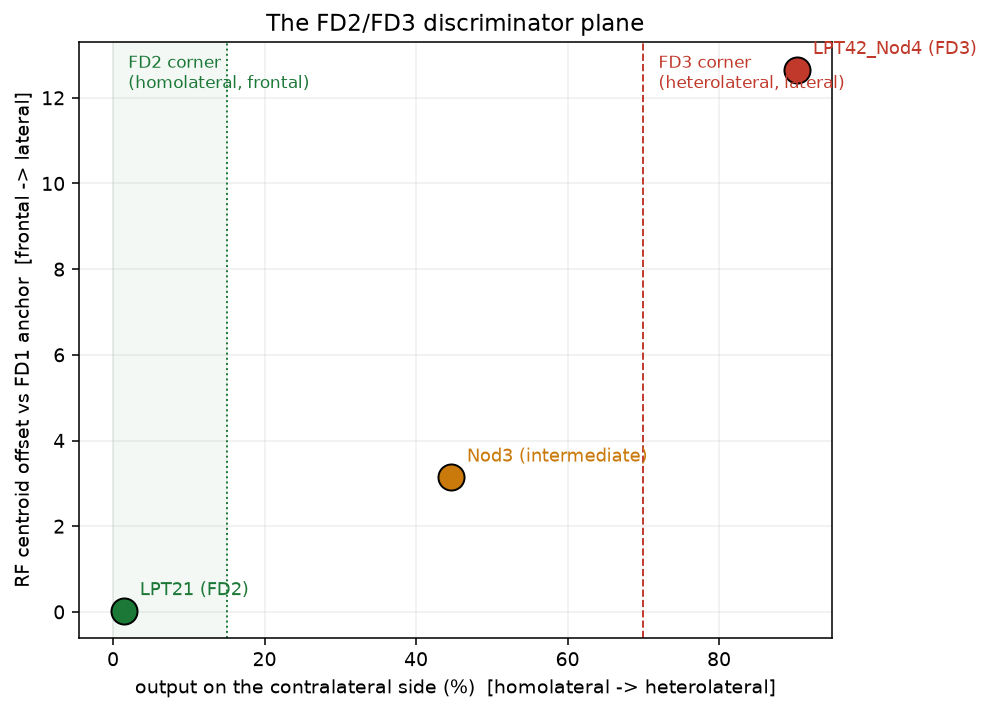
\includegraphics[width=\textwidth]{figures/fd3_disambig_fd2.png}
\caption{\textbf{The FD2/FD3 plane.} Each candidate placed by output laterality (horizontal, homolateral to heterolateral) and receptive-field offset from FD1 (vertical, frontal to lateral). \ttt{LPT21} sits in the FD2 corner (homolateral, frontal); \ttt{LPT42\_Nod4} in the FD3 corner (heterolateral, lateral); \ttt{Nod3} between them.}\label{fig:plane}
\end{figure}


\paragraph{The axon morphology agrees with the projection count.} Reconstructing each cell's shape and separating the input (dendritic) from the output (axonal) field shows a medio-lateral shift in every cell, so the shift direction alone does not assign them; what does is how much output lands on the far side. The \ttt{LPT42\_Nod4} axon is displaced across the midline and its output is predominantly contralateral; the \ttt{LPT21} and \ttt{Nod3} axons stay on their own side by output count (Fig.~\ref{fig:morph}).

\begin{figure}[H]\centering
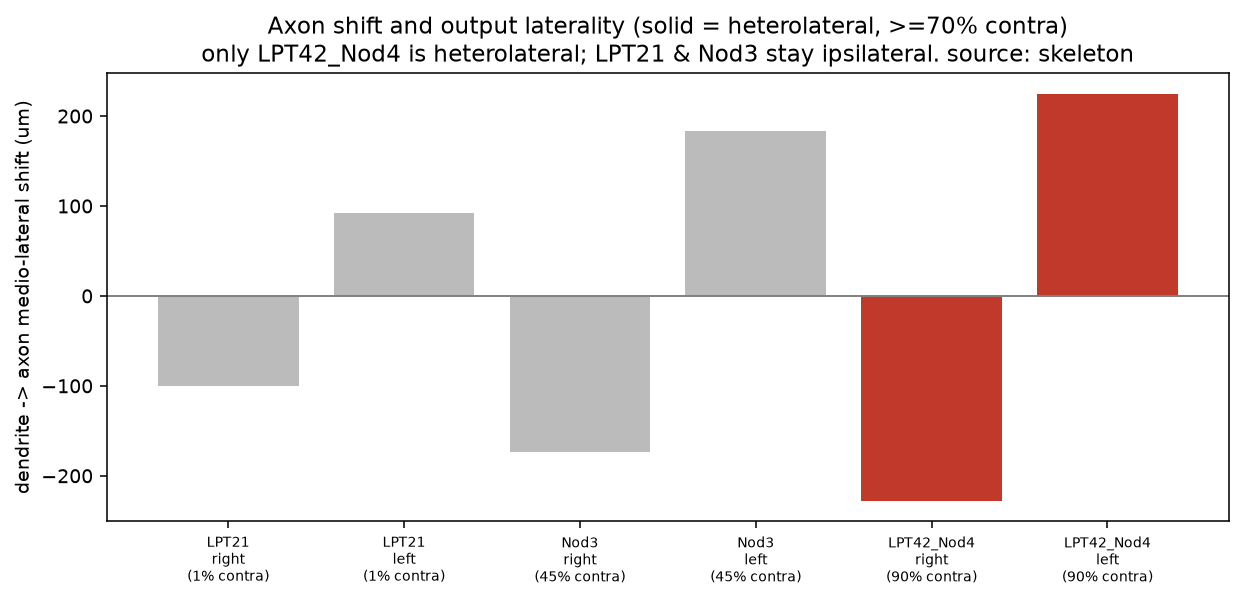
\includegraphics[width=\textwidth]{figures/fd3_disambig_morphology.png}
\caption{\textbf{Axon shift and output laterality.} The dendrite-to-axon medio-lateral shift per cell, with the contralateral output fraction noted beneath. Bars are solid where the cell is heterolateral (at least $70\%$ contralateral); only \ttt{LPT42\_Nod4} is. \ttt{LPT21} and \ttt{Nod3} keep their output ipsilateral.}\label{fig:morph}
\end{figure}


\paragraph{The whole-family feature match, and where it needs refining.} Scoring every candidate against all four FD cells on three binary features (direction, the lateral field with a gap, and the crossing axon) makes \ttt{LPT42\_Nod4} the reciprocal-best FD3 (Fig.~\ref{fig:heatmap}). For FD2 the binary score alone is not decisive: it rates both \ttt{LPT21} and \ttt{Nod3} at the FD2 signature, because it collapses every cell below the heterolateral cut-off into one category and so cannot see that \ttt{LPT21} is cleanly homolateral while \ttt{Nod3} is mixed. Resolving the tie on the finer measurements, the homolateral projection and the frontal co-location, selects \ttt{LPT21} as FD2 and leaves \ttt{Nod3} intermediate. As a check that the feature set can separate the FD cells, the FD1 anchor \ttt{Nod1} scores best for FD1 (FD1).

\begin{figure}[H]\centering
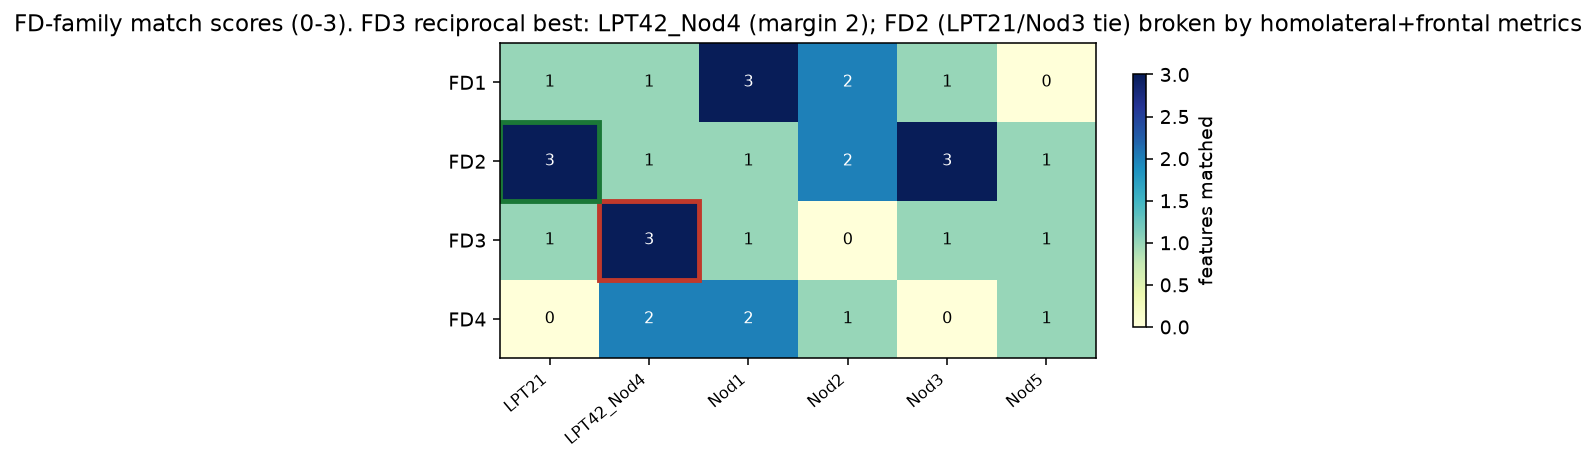
\includegraphics[width=\textwidth]{figures/fd3_family_heatmap.png}
\caption{\textbf{The family feature match.} Each candidate (columns) scored against each FD cell (rows) by shared binary features (0--3). \ttt{LPT42\_Nod4} (red outline) is the best match for FD3. The FD2 row scores \ttt{LPT21} (green outline) and \ttt{Nod3} equally on the binary features; the tie is broken toward \ttt{LPT21} by the finer homolateral and frontal-co-location measurements.}\label{fig:heatmap}
\end{figure}


\begin{figure}[H]\centering
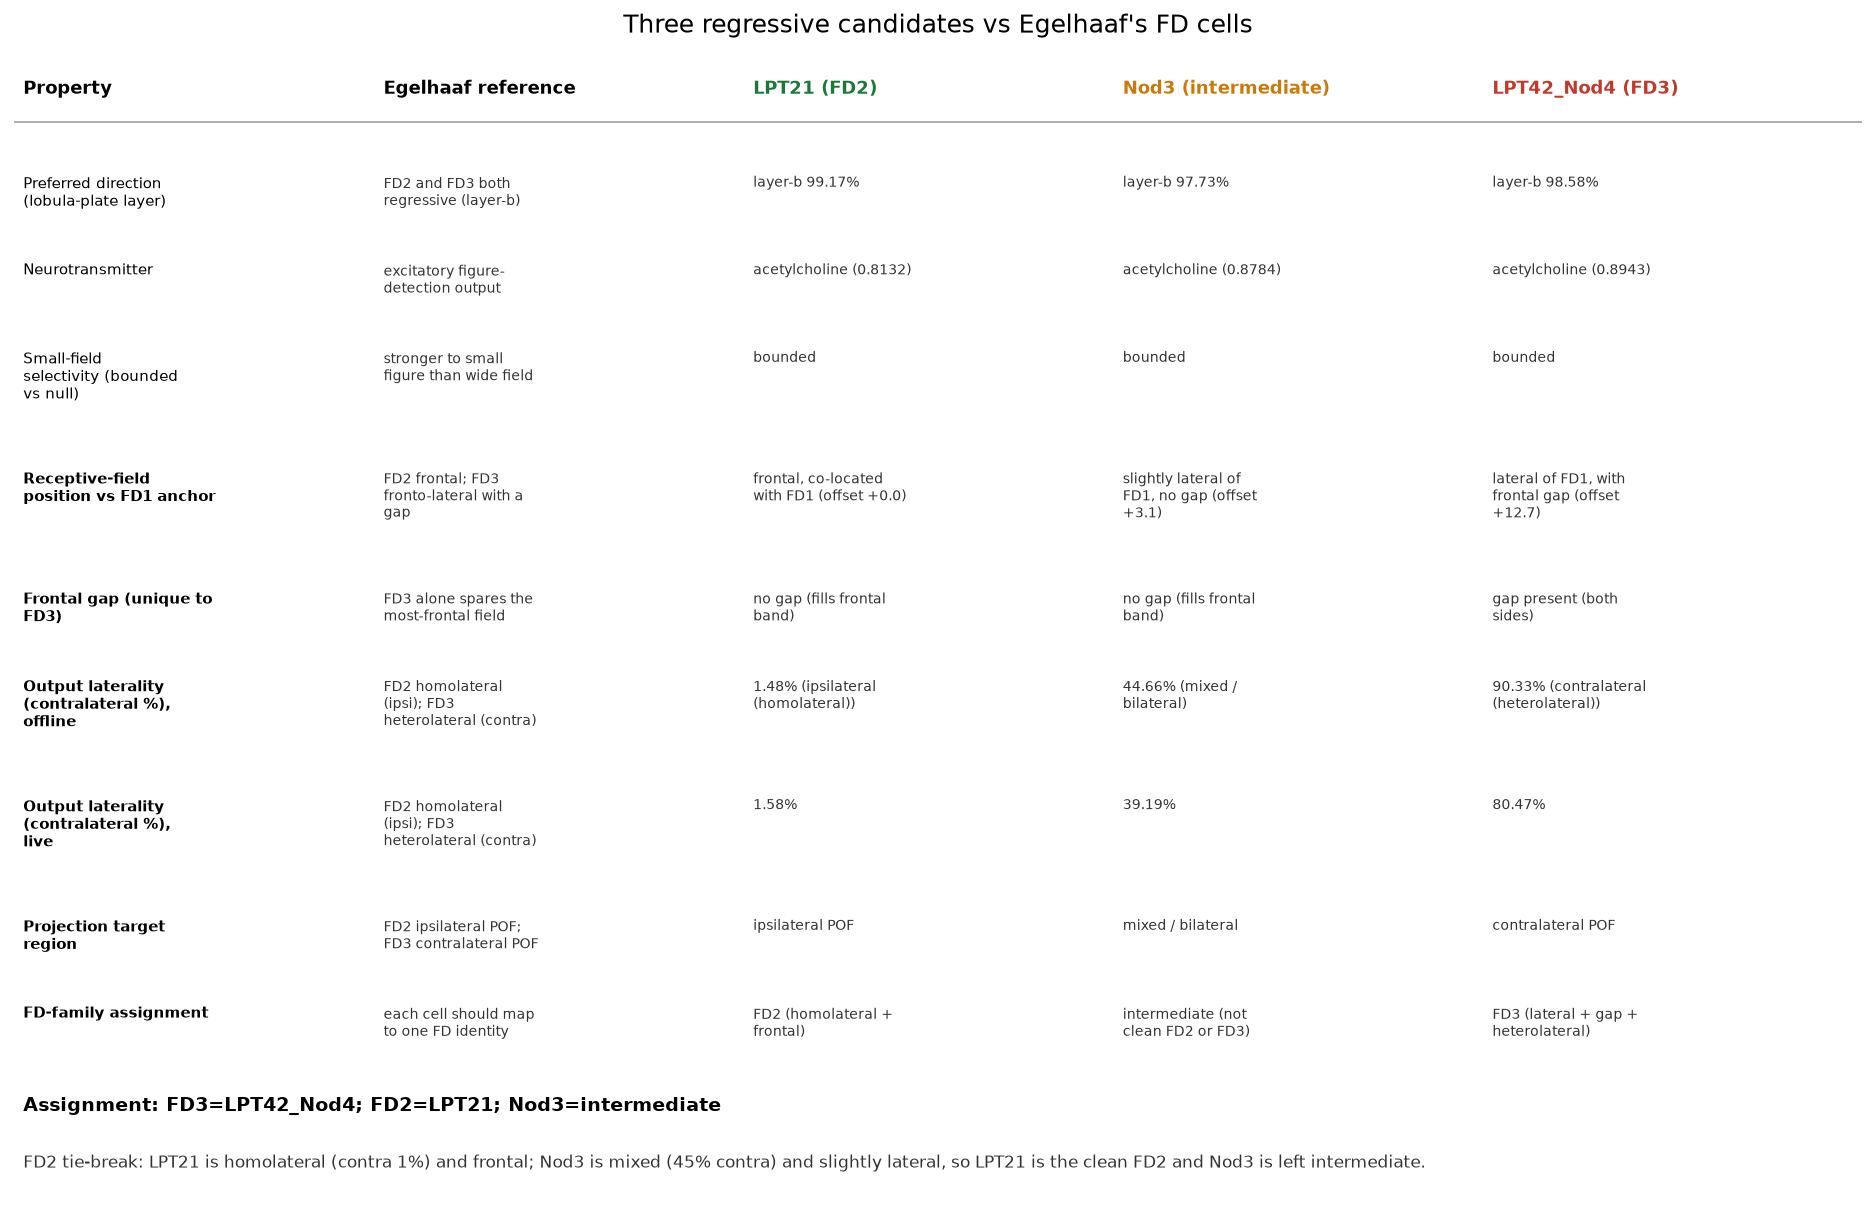
\includegraphics[width=\textwidth]{figures/fd3_disambig_decision.png}
\caption{\textbf{The three-way assignment, at a glance.} Each property, the Egelhaaf reference, and the measured value for each candidate. The shared properties (top) assign none; the projection and receptive-field rows place \ttt{LPT21} at FD2, \ttt{LPT42\_Nod4} at FD3, and \ttt{Nod3} between them.}\label{fig:decision}
\end{figure}


\section{\ttt{Nod3} is an intermediate regressive cell}

The earlier version of this analysis, comparing only \ttt{Nod3} and \ttt{LPT42\_Nod4}, assigned \ttt{Nod3} to FD2 because it is regressive and not FD3. Adding \ttt{LPT21} shows that assignment was too quick. On the two axes that define FD2, \ttt{LPT21} is a clean match and \ttt{Nod3} is not. \ttt{Nod3}'s output is 44.66\% contralateral, neither the near-zero of a homolateral FD2 cell nor the high fraction of a heterolateral FD3 cell, and its receptive field is displaced only slightly from the front, between FD2's frontal field and FD3's lateral field. \ttt{Nod3} is therefore best described as an intermediate regressive noduli-family figure cell: it belongs to the same functional group but does not match a single one of Egelhaaf's described FD cells. Whether it is a distinct cell Egelhaaf did not record, a variant of one he did, or a graded member of the regressive set is a question the wiring alone does not settle, and it is left open here rather than forced.

\section{The evidence at a glance}

Table~\ref{tab:disambig} collects every property next to the measured value for each of the three candidates. The shared properties assign none; the projection and receptive-field rows place \ttt{LPT21} at FD2, \ttt{LPT42\_Nod4} at FD3, and \ttt{Nod3} between them.

\begin{table}[H]\centering\footnotesize\caption{The three regressive candidates against Egelhaaf's FD reference properties. Direction and transmitter are shared; output laterality and receptive-field position assign \ttt{LPT21} to FD2 (frontal, homolateral), \ttt{LPT42\_Nod4} to FD3 (lateral with a gap, heterolateral), and leave \ttt{Nod3} intermediate.}\label{tab:disambig}

\renewcommand{\arraystretch}{1.2}
\setlength{\tabcolsep}{3pt}
\begin{longtable}{@{}>{\raggedright\arraybackslash}p{0.17\textwidth} >{\raggedright\arraybackslash}p{0.21\textwidth} >{\raggedright\arraybackslash}p{0.20\textwidth} >{\raggedright\arraybackslash}p{0.20\textwidth} >{\raggedright\arraybackslash}p{0.20\textwidth}@{}}
\toprule \textbf{Property} & \textbf{Egelhaaf reference} & \textbf{\ttt{LPT21} (FD2)} & \textbf{\ttt{Nod3} (interm.)} & \textbf{\ttt{LPT42\_Nod4} (FD3)} \\\midrule\endhead
Preferred direction (lobula-plate layer) & FD2 and FD3 both regressive (layer-b) & layer-b 99.17\% & layer-b 97.73\% & layer-b 98.58\% \\
Neurotransmitter & excitatory figure-detection output & acetylcholine (0.8132) & acetylcholine (0.8784) & acetylcholine (0.8943) \\
Small-field selectivity (bounded vs null) & stronger to small figure than wide field & bounded & bounded & bounded \\
Receptive-field position vs FD1 anchor & FD2 frontal; FD3 fronto-lateral with a gap & frontal, co-located with FD1 (offset +0.0) & slightly lateral of FD1, no gap (offset +3.1) & lateral of FD1, with frontal gap (offset +12.7) \\
Frontal gap (unique to FD3) & FD3 alone spares the most-frontal field & no gap (fills frontal band) & no gap (fills frontal band) & gap present (both sides) \\
Output laterality (contralateral \%), offline & FD2 homolateral (ipsi); FD3 heterolateral (contra) & 1.48\% (ipsilateral (homolateral)) & 44.66\% (mixed / bilateral) & 90.33\% (contralateral (heterolateral)) \\
Output laterality (contralateral \%), live & FD2 homolateral (ipsi); FD3 heterolateral (contra) & 1.58\% & 39.19\% & 80.47\% \\
Projection target region & FD2 ipsilateral POF; FD3 contralateral POF & ipsilateral POF & mixed / bilateral & contralateral POF \\
FD-family assignment & each cell should map to one FD identity & FD2 (homolateral + frontal) & intermediate (not clean FD2 or FD3) & FD3 (lateral + gap + heterolateral) \\
\bottomrule\end{longtable}
\renewcommand{\arraystretch}{1.0}
\setlength{\tabcolsep}{6pt}

\end{table}

\section{What the data can and cannot settle}

\textbf{Each cell type is one bilateral pair.} \ttt{LPT21}, \ttt{Nod3} and \ttt{LPT42\_Nod4} are each a single left/right pair, which is how many the fly has. The result rests on the two cells of each pair agreeing, on the comparison against the FD1 anchor, and on resampling the thousands of synapses each cell carries, not on a population average. \textbf{The contralateral fraction is data-source sensitive.} The exact percentage moves between the offline, live and v630 tracks because unannotated local fragments are excluded from the count (the track-to-track movement for \ttt{LPT42\_Nod4} is about 9.9 percentage points); the ordering of the three candidates is preserved on every track, so the assignment does not depend on any one of them. \textbf{FD2's large-field organisation was not measured.} Egelhaaf reports that FD2's large-field input could not be resolved, so FD2's only documented properties are its frontal field and its ipsilateral projection; the FD2 assignment of \ttt{LPT21} rests on those two, not on a contralateral property. \textbf{Absolute visual angle is approximate.} The receptive-field argument is built on the relative comparison to the frontal FD1 cell and does not rely on absolute azimuth. \textbf{\ttt{Nod3}'s positive identity is left open.} It is regressive and a figure cell, but the data place it between FD2 and FD3 rather than on either, and it is reported as an intermediate rather than assigned.

\section{Methods and provenance}

\textbf{Connectome.} FlyWire FAFB materialization v783 (\ttt{synapses\_nt\_v1}, no cleft threshold), offline track as the primary source, with the live v783 and v630 tracks confirming the laterality measurements. Neuron annotations (cell type, side, super-class, neurotransmitter and confidence, soma coordinates) are the Schlegel/Codex tables. \textbf{Preferred direction} is the synapse-weighted T4/T5 lobula-plate layer composition (layer$\to$direction after Fischbach \& Dittrich and Maisak et al.~\cite{fd1989,maisak2013}). \textbf{Output laterality} is the fraction of a cell's output synapses whose postsynaptic partner lies on the opposite side of the brain, reported per track and read as a continuum (homolateral near zero, heterolateral high). \textbf{Receptive field}: each cell's T4/T5 inputs carry hex-lattice (p,q) coordinates; the differential test compares the synapse-weighted centroid and frontal-band occupancy against the FD1=\ttt{Nod1} anchor, with a 2000-sample within-cell bootstrap, and the axis convention is pinned by a self-test requiring the known-frontal FD1 anchor to land frontal. \textbf{Morphology}: input and output synapse positions and reconstructed skeletons give the dendrite and axon fields. \textbf{Family match}: a binary feature-match over the Nod/LPT \ttt{visual\_projection} types against the four FD signatures, with the FD2 tie between \ttt{LPT21} and \ttt{Nod3} resolved on the homolateral and frontal-co-location measurements. \textbf{Reproducibility}: all randomness is seeded (12345). The report is built from the disambiguation JSON. Primary track: \ttt{offline}.

\begin{thebibliography}{9}
\bibitem{egelhaaf1985a} Egelhaaf M. (1985) On the neuronal basis of figure-ground discrimination by relative motion in the visual system of the fly. I. \textit{Biol. Cybern.} 52:123--140.
\bibitem{egelhaaf1985b} Egelhaaf M. (1985) \ldots II. Figure-detection cells, a new class of visual interneurones. \textit{Biol. Cybern.} 52:195--209. (FD2 at p.~201; FD3 at pp.~202--204.)
\bibitem{egelhaaf1985c} Egelhaaf M. (1985) \ldots III. Possible input circuitries and behavioural significance of the FD-cells. \textit{Biol. Cybern.} 52:267--280.
\bibitem{rp1979} Reichardt W., Poggio T. (1979) Figure-ground discrimination by relative movement in the visual system of the fly. I. \textit{Biol. Cybern.} 35:81--100.
\bibitem{fd1989} Fischbach K.-F., Dittrich A.P.M. (1989) The optic lobe of \textit{Drosophila melanogaster}. I. A Golgi analysis of wild-type structure. \textit{Cell Tissue Res.} 258:441--475.
\bibitem{maisak2013} Maisak M.S. et al. (2013) A directional tuning map of \textit{Drosophila} elementary motion detectors. \textit{Nature} 500:212--216.
\bibitem{dorkenwald2024} Dorkenwald S. et al. (2024) Neuronal wiring diagram of an adult brain. \textit{Nature} 634:124--138.
\bibitem{schlegel2024} Schlegel P. et al. (2024) Whole-brain annotation and multi-connectome cell typing of \textit{Drosophila}. \textit{Nature} 634:139--152.
\bibitem{codex} FlyWire Codex, \texttt{codex.flywire.ai} -- cell-type and annotation portal.
\end{thebibliography}

\end{document}